\begin{verbatim}
  * Impact on performance (IPC)
  * Impact on energy
  * Coverage
  * Deep Dive
    * Cache characterization 
        Locality impact?
    * Slice statistics 
        Instruction mix, length, ...
    * Recomputation overhead?
    * Sensitivity analysis?
    * ...
 \end{verbatim}

\begin{figure}[t]
  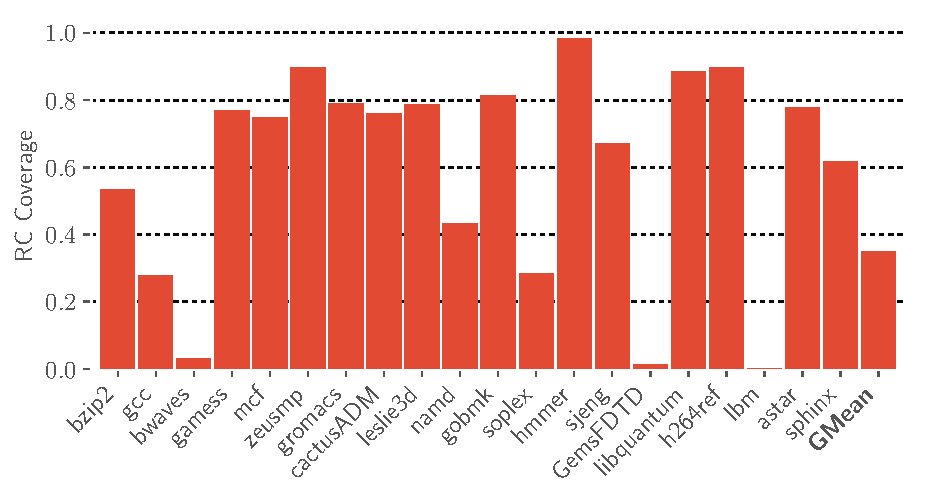
\includegraphics[width=\columnwidth]{figs/rc_coverage.pdf}
  \caption{The coverage of the \recomp, i.e. the ratio of shadowed L1 misses that can be recomputed instead of being delayed.}
  \label{fig:rc-coverage}
\end{figure}

\begin{figure}[t]
  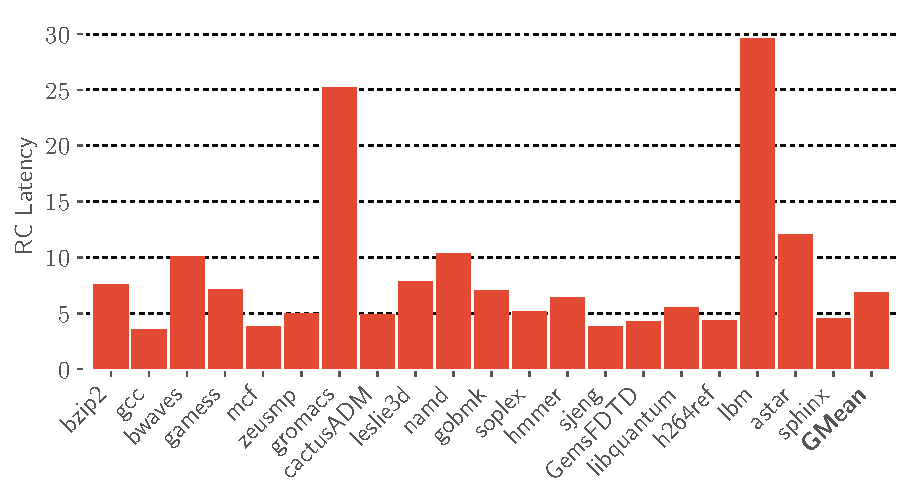
\includegraphics[width=\columnwidth]{figs/rc_latency.pdf}
  \caption{The average latency for recomputing a shadowed L1 miss.}
  \label{fig:rc-latency}
\end{figure}

\begin{figure*}[t]
  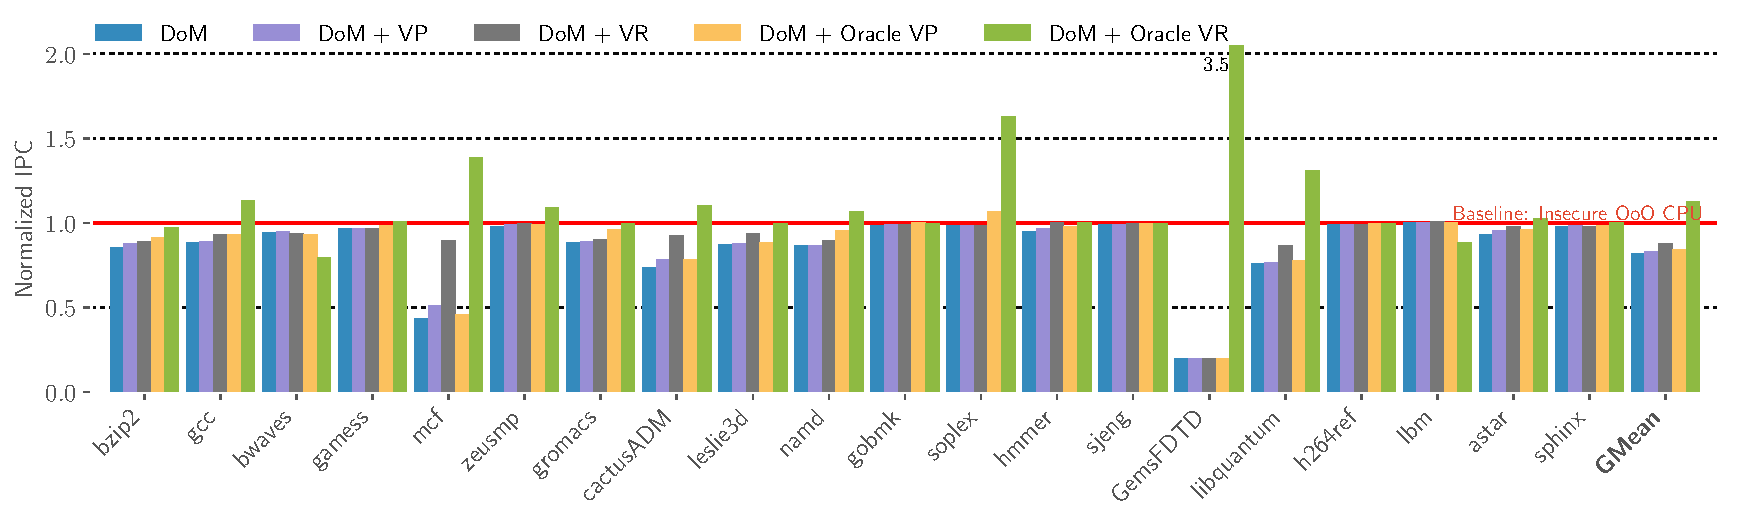
\includegraphics[width=\textwidth]{figs/normalized_ipc_cut_all.pdf}
  \caption{Performance (IPC -- higher is better) normalized to an insecure OoO baseline.}
  \label{fig:ipc}
\end{figure*}

\begin{figure*}[t]
  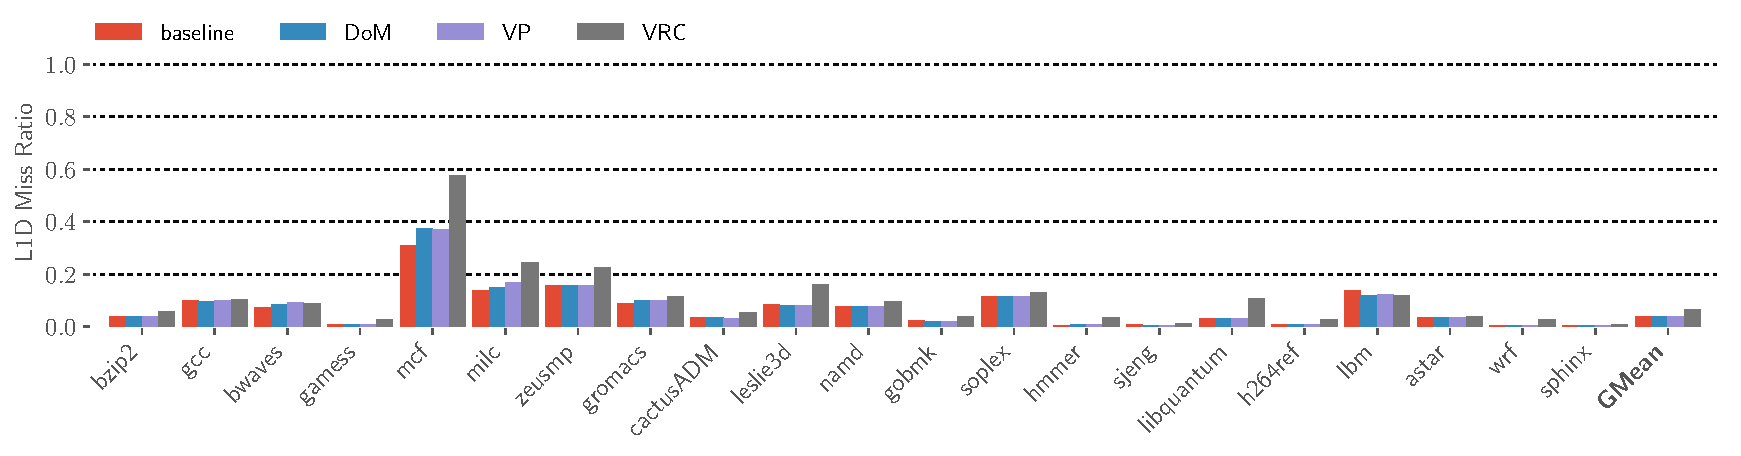
\includegraphics[width=\textwidth]{figs/l1d_miss_ratio.pdf}
  \caption{L1D miss ratio for Delay-on-Miss with VR and \recomp.}
  \label{fig:l1d_misses}
\end{figure*}

\begin{figure*}[t]
  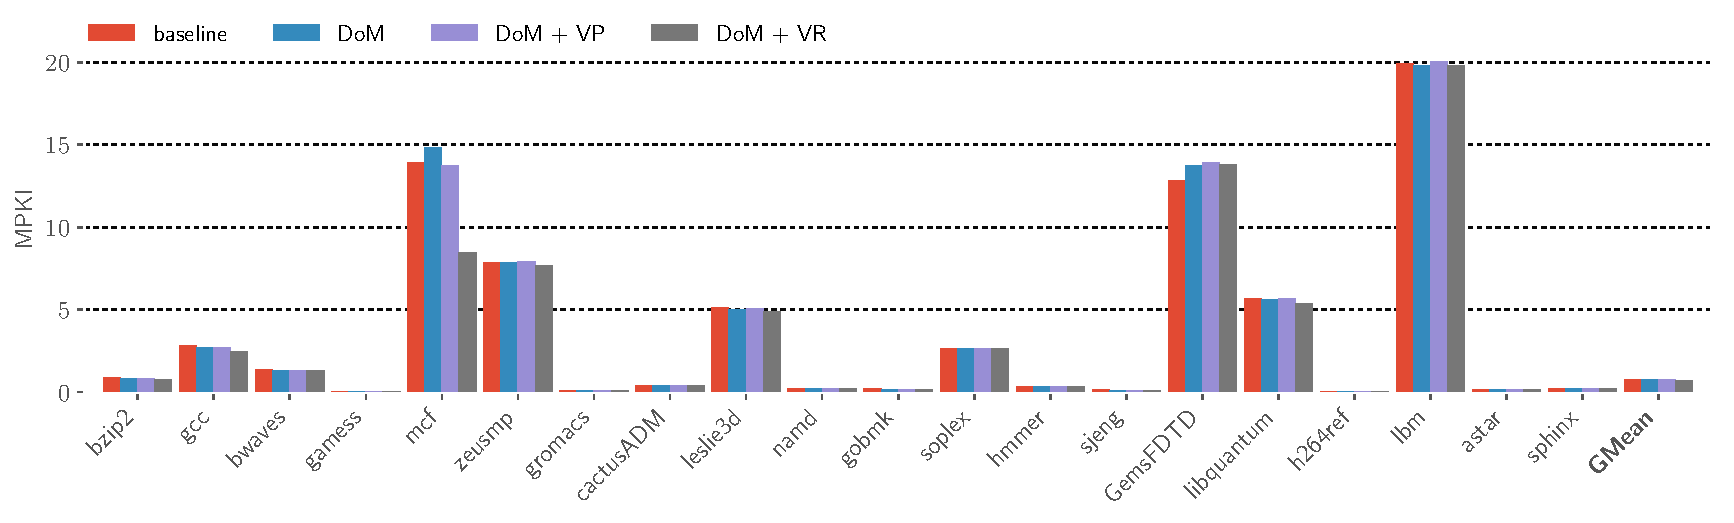
\includegraphics[width=\textwidth]{figs/mpki.pdf}
  \caption{LLC misses per 1000 instructions (MPKI).}
  \label{fig:mpki}
\end{figure*}

\begin{figure*}[t]
  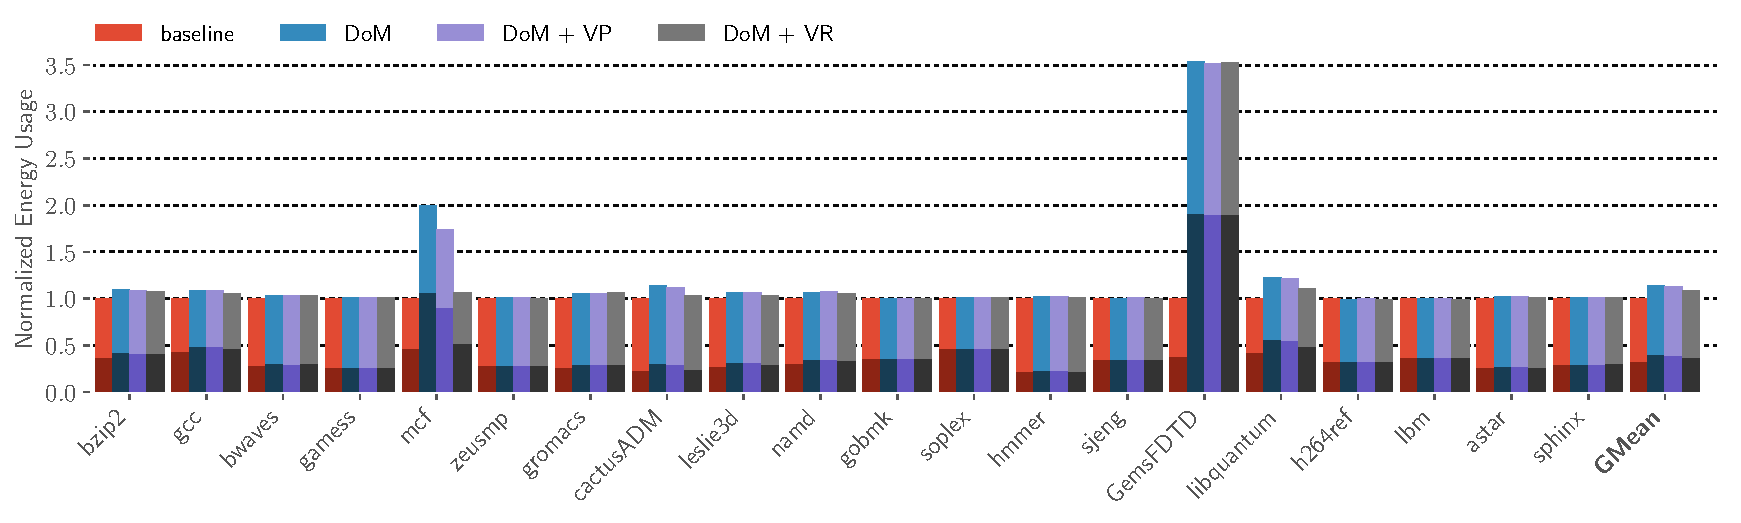
\includegraphics[width=\textwidth]{figs/normalized_energy_usage.pdf}
  \caption{Energy usage for the different approaches. The darker, bottom part of each bar represents the static energy usage, while the lighter, top part represents the dynamic.}
  \label{fig:energy}
\end{figure*}

\subsection{Performance}
\label{sec:performance}

~\autoref{fig:ipc} contains the number of instructions committed successfully per cycle, normalized to the insecure baseline processor. Delay-on-Miss with VP or \recomp, which is our \emph{secure} baseline, performs at $82\%$ of the baseline, similarly to the results reported by Sakalis et al. The two benchmarks that incur the biggest hit in performance are \texttt{GemsFDTD} (at $20\%$ of the baseline), \texttt{mcf} ($44\%$), followed by \texttt{cactusADM} ($74\%$) and \texttt{libquantum} ($76\%$). All of these benchmarks have high MPKI (\autoref{fig:mpki}), but that in itself is not the only factor, as other benchmarks (e.g. \texttt{lbm}) also have high MPKI. Instead, the cost of DoM also depends on the amount of MLP that the benchmarks exhibit; the more the MLP taken advantage of in the baseline, the higher the performance loss. This is particularly true for \texttt{GemsFDTD}, which is one of the benchmarks with a large number of concurrent long latency loads to multiple cache lines.

If VP is introduced, then the performance is similar, at $83\%$ of the baseline.
This result contradicts the results given by Sakalis et al., where the VP gives a significant performance advantage. We have contacted them and verified that our results are indeed valid. %TODO: This should be rewritten when we are no longer anonymous
The reason that VP does not offer a significant advantage is because VP itself is speculative: When a value is predicted it still needs to be validated at a later point. By predicting the value, a small amount of parallelism can be exploited during execution, but the slow L1 misses still need to be satisfied for the validation. Due to the M- and the VP-shadows, validations have to be serialized and are not able to take advantage of any MLP that might be found in the application. In essence, the VP pushes the cost of delaying speculative loads from the execution stage to the validation stage, but it does not eliminate it. This can be seen in the Oracle VP results, where even $100\%$ prediction rate (i.e. all shadowed L1 misses are successfully predicted) only leads to a marginal performance improvement of one percentage point.

On the other hand, the same is not true for \recomp, which is not speculative. Once a value has been recomputed, it does not need to be validated, meaning that the cost for delaying a long latency miss does not need to be payed, nor is there any serialization enforced. While \recomp~ does not really increase the amount of MLP that can be taken advantage of, it does eliminate some the need for it. Overall, \recomp~ performs at $88\%$ of the baseline, decreasing the performance cost of DoM by one third. The benchmark with the most dramatic performance increase is \texttt{mcf}, the second worse performing benchmark for DoM. \recomp~ improves the performance from $44\%$ to $90\%$, reducing the performance cost to one fifth of that of DoM. As a matter of fact, \recomp performs better or equal to VP for every single benchmark we have evaluated. \redHL{Unfortunately, in the case of \texttt{GemsFDTD}, we have a very low slice coverage, meaning that most of the loads cannot be recomputed.} Because of this, \recomp, much like VP, does not improve the performance over DoM.

If we introduce an Oracle \recomp~ that can recompute all shadowed L1 misses, the difference between the VP and the \recomp~ approaches becomes even more apparent. With both Oracles having $100\%$ coverage, the main difference is if the loads need to be validated once they are unshadowed (VP) or not (\recomp). 
With the \recomp~ Oracle, even though the latency for getting a value is higher than than of the VP Oracle, we are able to outperform of even the insecure baseline. Of course, such an Oracle is unrealistic, but it does support our argument that the big limitation of VP is the cost of validation. Additionally, given the $3.5\times$ over the baseline performance improvement we can observe in \texttt{GemsFDTD}, it further validates our analysis that \texttt{GemsFDTD} suffers from a lot of long latency misses that require a lot of MLP to hide.

\subsection{Energy Efficiency}
\label{sec:energy}

Energy efficiency, in our case, is affected by three main factors: The execution time/performance, the number of accesses in the memory hierarchy (especially the DRAM), and the cost of predicting or recomputing a value.
~\autoref{fig:energy} contains the combined static and dynamic energy usage of the system. It is immediately obvious that the two benchmarks that have the worst execution performance are also the two benchmarks that have the worst energy usage. While overall DoM, VP, and \recomp~ increase the mean energy usage over the baseline by $14\%$, $13\%$, and $9\%$ respectively, \texttt{GemsFDTD} and \texttt{mcf} incur a $3.5\times$ and $2\times$ performance overhead respectively. As previously discussed in the performance analysis (~\autoref{sec:performance}), \recomp~ does not improve the results for \texttt{GemsFDTD} due to low coverage, but it does decrease the overhead for \texttt{mcf} to just $6\%$ over the baseline. This is a combination of both reducing the execution time and reducing the MPKI/DRAM accesses. In contrast, the VP incurs an overhead $1.7\times$ over the baseline.

\subsection{Memory Behavior}
\label{sec:memory}